\section{Problem Solution}
\label{sec:solution}

We will make use of Figure~\ref{fig:solution} in the following derivation.
The diagonal length $d \triangleq \abs{AC}$ of the rectangle is given by 
%
\begin{equation}
  d^2 = w^2 + h^2.
  \label{eq:diagsq}
\end{equation}
%
\begin{figure}[h]
  \centering
  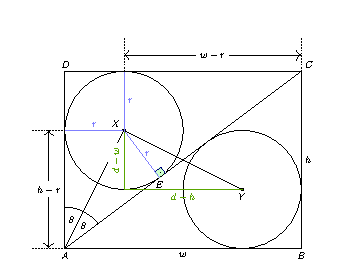
\includegraphics[trim={0 0 0 0.55cm},clip,width=0.5\textwidth]{./figures/basic2.pdf}
  \vspace{-8mm}
  \caption{Auxiliary drawing, identifying key lengths and angles.}
  \label{fig:solution}
\end{figure}
%
The diagonal length $d$ may also be related to $(w,h)$ and $r$ by noting that
$\abs{AE} = h-r$ and $\abs{EC} = w-r$ due to the tangency to the circles. On the
other hand, $d = \abs{AC} = \abs{AE} + \abs{EC}$ so that 
%
\begin{equation}
  d + 2r = w + h.
  \label{eq:diaglin}
\end{equation}

\subsection{Computing $\abs{XY}$ and $r$, given $w$ and $h$}
\label{ssec:compute_xyr}

In order to compute $\abs{XY}$, form the right triangle whose horizontal and
vertical sides are drawn in green in Figure~\ref{fig:solution}. The length of
the vertical side of this triangle is $h-2r$ but by equation~\eqref{eq:diaglin}
this is equal to $d-w$. Similarly, the length of the horizontal side of this
triangle is $w-2r$ but, by the same token, this is equal to $d-h$. Hence, we
have
%
\begin{equation}
  \abs{XY}^2 = (d-w)^2 + (d-h)^2 = 3d^2 - 2d(w+h),
  \label{eq:xylen}
\end{equation}
%
where the second equality may be derived by substituting from
equation~\eqref{eq:diagsq}. The radius $r$ can be read off from
equation~\eqref{eq:diaglin}.
%
\begin{equation}
  r = \nicefrac{1}{2}(w+h-d)
  \label{eq:radius}
\end{equation}

\subsection{Computing $f$ and its inverse $f^{-1}$}

The computation in the previous section determines $f:
\mathbb{R}_+^2 \rightarrow \mathbb{R}_+^2$.
%
\begin{align}
  \begin{split}
    d &= \sqrt{w^2 + h^2}, \\
    f(w,h) &= \left( \nicefrac{1}{2}(w+h-d), \sqrt{(d-w)^2 + (d-h)^2} \right).
  \end{split}
  \label{eq:f}
\end{align}
%
In order to look for its inverse, let us recall equation~\eqref{eq:xylen} and
substitute from~\eqref{eq:diaglin} for $w+h$, yielding the relationship 
\begin{equation} 
 d^2 - 4rd - \abs{XY}^2 = 0, 
 \label{eq:dquad}
\end{equation}
%
which implies 
%
\begin{equation}
  d = 2r + \sqrt{\abs{XY}^2 + 4r^2}, 
  \label{eq:inversed}
\end{equation}
%
since $d > 0$. Let us solve for $h$ from equation~\eqref{eq:diaglin} and
substitute into equation~\eqref{eq:diagsq}, which yields \[ w^2 - (2r+d)w +
2r(r+d) = 0. \] Now, if we notice that equations~\eqref{eq:diagsq}
and~\eqref{eq:diaglin} are both symmetric in $w$ and $h$, then we can deduce
that the two solutions of this quadratic equation correspond to $w$ and $h$.
Assuming, without loss of generality, $w > h$, and substituting
from~\eqref{eq:dquad} and~\eqref{eq:inversed}, we obtain 
%
\begin{align*}
  w(r,\abs{XY}) &= \nicefrac{1}{2}\left(2r+d + \sqrt{d^2 - 4rd - 4r^2} \right) \\ 
    &= 2r + \nicefrac{1}{2} \left( \sqrt{\abs{XY}^2 + 4r^2} + \sqrt{\abs{XY}^2 -
4r^2} \right),
\end{align*}
%
and 
%
\begin{align*}
  h(r,\abs{XY}) &= \nicefrac{1}{2}\left(2r+d - \sqrt{d^2 - 4rd - 4r^2} \right) \\ 
    &= 2r + \nicefrac{1}{2} \left( \sqrt{\abs{XY}^2 + 4r^2} - \sqrt{\abs{XY}^2 -
4r^2} \right),
\end{align*}
%
which yields the inverse function $f^{-1}(r,\abs{XY}) = (w,h)$.
